Totem jest prostym odtwarzaczem filmów. Dwukrotne kliknięcie pliku wideo w menadżerze plików uruchomi jego odtwarzanie w programie Totem. Zaznaczenie i próba otwarcia wielu filmów w menadżerze plików spowoduje dodanie ich do kolejki odtwarzania. 

Totem korzysta z zainstalowanych w systemie kodeków. Jeżeli postępując zgodnie z tym przewodnikiem zainstalowałeś pakiet \textcolor{ubuntu_orange}{ubuntu-restricted-extras}, to Totem będzie w stanie odtworzyć każdy popularny format wideo.
\begin{center}
	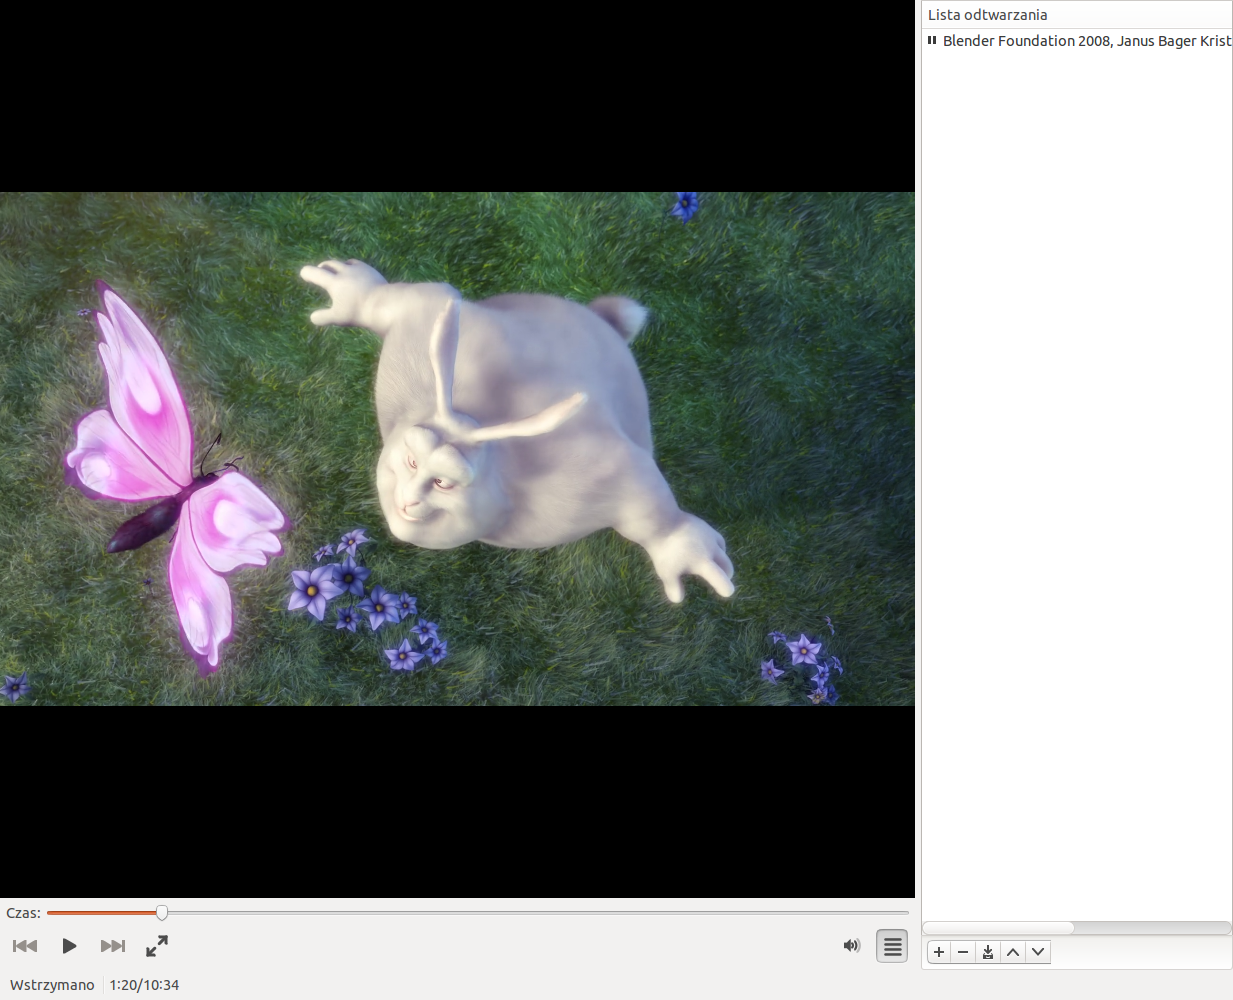
\includegraphics[width=\linewidth]{images/programy_totem1.png}
\end{center}

\subsubsection{Podstawy obsługi programu Totem}
Otwieranie plików:
\begin{itemize}
\item Wybierz \menu{{Film}>{Otwórz\ldots}}, aby wskazać plik na lokalnym dysku.
\item Wybierz \menu{{Film}>{Otwórz z położenia\ldots}}, aby wskazać plik w internecie, który ma zostac pobrany i odtworzony. Link do pliku musi być absolutny, tzn. wskazywać bezpośrednio film, a nie stronę z filmem.
\end{itemize}
Oglądanie filmu:
\begin{itemize}
\item Dwukrotne kliknięcie w obszarze oglądanego filmu uruchomi tryb pełnoekranowy.
\item Klawisz \keys{\Space} wstrzymuje/wznawia odtwarzanie.
\item Klawisz \keys{\arrowkeyright} przeskakuje jedną minutę do przodu.
\item Klawisz \keys{\arrowkeyleft} przeskakuje 15 sekund do tyłu.
\item Kółko myszy także pozwala na przemieszczanie się po filmie, o ile kursor myszy znajduje się nad obszarem odtwarzania.
\item Aby załadować napisy, wybierz \menu{{Widok}>{Napisy}>{Wybierz plik z napisami}}.
\end{itemize}

\subsubsection{Automatyczna obsługa napisów}
Gdy program jest włączony, z panelu menu wybierz \menu{Edycja>Preferencje>Ogólne>} i zaznacz ,,Wczytywanie pliku napisów po wczytaniu filmu'', zmień domyślną czcionkę na \textit{FreeSans.ttf} oraz ustaw kodowanie na ,,środkowoeuropejskie (WINDOWS-1250)''. Jeśli plik z napisami będzie miał taką samą nazwę, jak nazwa pliku z filmem, napisy zostaną załadowane automatycznie.
